\subsubsection{Double mach reflection}
\label{sec.tests.doublemach}

The double mach reflection test is a classic two-dimensional test of
hydrodynamic algorithms originally described in
\citet{1984JCoPh..54..115W} \citep[and more recently
in][]{2008ApJS..178..137S}.  In this problem, shown in
Figure~\ref{fig.doublemach}, a shock is injected at an angle to a
reflecting surface (the -y boundary), and a jet appears along the
reflecting surface.  The ideal solution is self-similar, and the
appearance of this solution is highly sensitive to numerical
diffusion.  If numerical noise is present, a Kelvin-Helmholz
instability develops along this jet and breaks the self-similarity.

In the test problem shown in Figure~\ref{fig.doublemach}, a 2D
simulation with $960 \times 240$ cells was created with a domain of $x
= [0, 4]$ and $y = [0, 1]$.  We use an ideal gas equation of state of
$\gamma = 1.4$, a pre-shock density of 1.4, and a pre-shock specific
internal energy of $2.5/1.4$ (all in arbitrary units).  A Mach 10
shock is initialized with a shock normal that is 30$^\circ$ from the
x-axis and an initial position on the lower boundary of x$ = 1/6$.
The lower y boundary and right x boundary are reflecting; the left x
boundary is inflowing, and the upper y boundary has a time-dependent
boundary condition that allows the shock to propagate into the domain
as if it extends to infinity.  The simulation starts at t$ = 0$ and
runs until t$ = 0.205$ (arbitrary units), at which point the rightmost
extent of the shock should be at roughly x$ = 3$.  In this simulation we use
the direct Eulerian implementation of the piecewise parabolic hydrodynamic
method with the diffusion, flattening, and shock steepening all enabled.

It is instructive to compare Figure~\ref{fig.doublemach} to Figure 9
in~\citet{1984JCoPh..54..115W}.  By the end of the simulation, a dense
jet is apparent at the leading edge of the shock, propagating along
the x-axis.  The shape of this jet is sensitive to numerical
diffusion, and our figure compares favorably to the higher-order
images from Woodward \& Colella.

\begin{figure}
\begin{center}
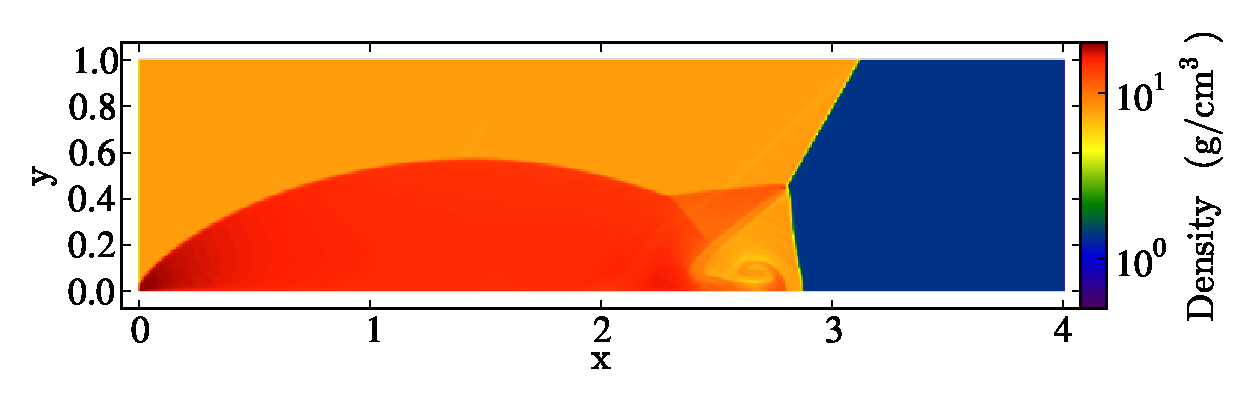
\includegraphics[width=0.8\textwidth]{figures/DoubleMachTest.eps}
\caption{Density field at the final time in the Double Mach test.  A
Mach 10 shock is injected into the domain with a shock normal that is
30$^\circ$ from the x-axis with a time-dependent +y boundary condition
that mimics a shock of infinite length.  The solution is self-similar,
with the jet and whorls at $x \simeq 2.5-3.0$ in this figure being very sensitive
to numerical diffusion.  Our results compare favorably to the
higher-order images from \citet{1984JCoPh..54..115W}.}
\label{fig.doublemach}
\end{center}
\end{figure}
